\documentclass{article}

\usepackage[english, russian]{babel}
\usepackage{geometry}
\usepackage{graphicx}
\usepackage{listings}
\usepackage{xcolor}
\usepackage[14pt]{extsizes}
\usepackage{amsmath}
\usepackage{setspace}
\usepackage{multirow}
\usepackage{tocloft}
\usepackage{indentfirst} 
\usepackage{lipsum}
\usepackage{caption}

\RequirePackage{cmap}
\RequirePackage[utf8]{inputenc}
\RequirePackage[T2A]{fontenc}
\captionsetup[figure]{name={Рисунок},labelsep=endash}
\captionsetup[table]{singlelinecheck=false, labelsep=endash}

\renewcommand{\cftsecleader}{\cftdotfill{\cftdotsep}}
\geometry{pdftex, left = 3cm, right = 1cm	, top = 2cm, bottom = 2cm}
\onehalfspacing

\setlength{\parindent}{1,25cm}
\lstdefinestyle{python}{
	language={Python},
	basicstyle=\footnotesize\ttfamily,
	numbers=left,
	frame=single,
	tabsize=4,	
	breaklines=true
}

\DeclareCaptionLabelSeparator{line}{\ --\ }
\DeclareCaptionFont{white}{\color{white}}
\DeclareCaptionFormat{listing}{\colorbox[cmyk]{0.43,0.35,0.35,0.01}{\parbox{\textwidth}{\hspace{15pt}#1#2#3}}}
\captionsetup[lstlisting]{
	labelsep=line
}

\begin{document}
\begin{titlepage}
	\newgeometry{pdftex, left=2cm, right=2cm, top=2.5cm, bottom=2.5cm}
	\fontsize{12pt}{12pt}\selectfont
	\noindent\begin{tabular}{|c|c|}	\hline
	\noindent\begin{minipage}{0.15\textwidth}
		
\includegraphics[width=\linewidth]{tools/logo.png}
	\end{minipage} &
	\noindent\begin{minipage}{0.85\textwidth}\centering
		\textbf{\newline Министерство науки и высшего образования Российской Федерации}\\
		\textbf{Федеральное государственное бюджетное образовательное учреждение высшего образования}\\
		\textbf{«Московский государственный технический университет имени Н.Э.~Баумана}\\
		\textbf{(национальный исследовательский университет)»}\\
		\textbf{(МГТУ им. Н.Э.~Баумана)}
	\end{minipage} \\
	\hline	\end{tabular}\newline\newline\newline
	\noindent ФАКУЛЬТЕТ \underline{«Информатика и системы управления»} \newline\newline
	\noindent КАФЕДРА \underline{«Программное обеспечение ЭВМ и информационные технологии»}\newline\newline\newline\newline\newline\newline

	\noindent\begin{minipage}{1.0\textwidth}\centering
		\Large\textbf{   ~~~ Лабораторная работа №2}\newline
		\textbf{по дисциплине «Анализ алгоритмов»}\newline\newline\newline\newline\newline
	\end{minipage}

	\noindent\textbf{Тема} \underline{Алгоритмы умножения матриц}\newline\newline
	\textbf{Студент} \underline{Тузов Даниил Александрович}\newline\newline
	\textbf{Группа} \underline{ИУ7-52Б}\newline\newline
	\textbf{Преподаватель} \underline{Кормановский Михаил Владимирович}
	
	\begin{center}
		\vfill
		Москва, \the\year ~г.
	\end{center}
	\restoregeometry
	\clearpage
\end{titlepage}

\renewcommand{\contentsname}{СОДЕРЖАНИЕ} 
\tableofcontents
\setcounter{page}{2}
\clearpage

\section*{ВВЕДЕНИЕ}
\addcontentsline{toc}{section}{ВВЕДЕНИЕ}
Во второй лабораторной работе по анализу алгоритмов рассматриваются алгоритмы умножения матриц: стандартный и
алгоритм Винограда. 

Целью лабораторной работы является оценка ресурсной эффективности алгоритмов умножения матриц.
Для достижения поставленной цели небходимо решить следующие задачи:
\begin{itemize}
	\item описать математическую основу стандартного алгоритма умножения матриц и алгоритма Винограда
	\item описать модель вычислений
	\item разработать алгоритмы умножения матриц: стандартный, Винограда и оптимизированный алгоритм Винограда
	в соответствии со своим вариантом
	\item выполнить оценку трудоемкости разработанных алгоритмов
	\item реализовать разработанные алгоритмы в программном обеспечении с двумя режимами работы --
	одиночного рассчета и массированного замера
	\item выполнить замеры процессорного времени выполнения реализации разработанных алгоритмов в зависимости от 
	варьируемого линейного размера матриц
	\item выполнить сравнительный анализ рассчитанных трудоемкостей и результатов замера процессорного времени
	выполнения реализаций трех алгоритмов с учетом лучшего и худшего случаев по трудоемкости
\end{itemize}


\clearpage\section{Аналитическая часть}
В этой части рассматриваются теоретические аспекты понятия умножения матриц стандартным алгоритмом и с помощью
алгоритма Винограда.

\subsection{Умножение матриц стандартным алгоритмом}
Пусть даны две матрицы A и B размерности $N \times M$ и $M \times K$ соответственно:
\begin{equation}
	A = \begin{pmatrix}
		a_{11} & a_{12} & \ldots & a_{1m}\\
		a_{21} & a_{22} & \ldots & a_{2m}\\
		\vdots & \vdots & \ddots & \vdots\\
		a_{n1} & a_{n2} & \ldots & a_{nm}
	\end{pmatrix},
	\quad
	B = \begin{pmatrix}
		b_{11} & b_{12} & \ldots & b_{1k}\\
		b_{21} & b_{22} & \ldots & b_{2k}\\
		\vdots & \vdots & \ddots & \vdots\\
		b_{m1} & b_{m2} & \ldots & b_{mk}
	\end{pmatrix},
\end{equation}

 \noindent тогда произведением матриц A и B называется матрица C размерностью $N \times K$:
 
 \begin{equation}
	C = \begin{pmatrix}
		c_{11} & c_{12} & \ldots & c_{1k}\\
		c_{21} & c_{22} & \ldots & c_{2k}\\
		\vdots & \vdots & \ddots & \vdots\\
		c_{n1} & c_{n2} & \ldots & c_{nk}
	\end{pmatrix},
\end{equation}

\noindent такая, что 
\begin{equation}
	\label{eq:M}
	c_{ij} =
	\sum_{k=1}^{m} a_{ik}b_{kj} \quad (i=\overline{1,N}; j=\overline{1,K})
\end{equation}


\subsection{Алгоритм Винограда}
В стандартном алгоритме для вычисления j-ого значения в i-ой строке результирующей матрицы необходимо поссчитать 
скалярное произведение i-ой строки $U = (u_1, u_2, u_3,..., u_n)$ первой матрицы на j-ый столбец $V = (v_1, v_2, v_3,..., v_n)$
второй матрицы, что равно $U \cdot V = u_1v_1 + u_2v_2 + u_3v_3 + ... + u_nv_n$.

Виноград в своем алгоритме предлагает другой способ вычисления скалярного произведения. Этот способ основан на
снижении доли операций умножения. Пусть есть два вектора $U = (u_1, u_2, u_3, u_4)$ и $V = (v_1, v_2, v_3, v_4)$, тогда их
скалярное произведение $U \cdot V = u_1v_1 + u_2v_2 + u_3v_3 + u_4v_4$, что эквивалентно (\ref{eq:vinograd}):
\begin{equation}
	\label{eq:vinograd}
	V \cdot W = (v_1 + w_2)(v_2 + w_1) + (v_3 + w_4)(v_4 + w_3) - v_1v_2 - v_3v_4 - w_1w_2 - w_3w_4.
\end{equation}

Произведения $v_1v_2$, $v_3v_4$, $w_1w_2$ и $w_3w_4$ можно поссчитать заранее, а затем использовать их при
вычислении значений в результирующей матрице.

\subsection{Вывод}
В этой части были рассмотрены теоретические аспекты алгоритмов умножения матриц. Основное отличие алгоритмов
заключается в способе вычисления скалярного произведения. В алгоритме Винограда выполняется предварительная обработка,
которая в дальнейшем помогает снизить долю операций умножения.


\clearpage\section{Конструкторская часть}
В этой части представлены описания алгоритмов, а также модель вычисления трудоемкостей алгоритмов.

\subsection{Описание алгоритмов}
На вход алгоритмам подаются две матрицы A и B. На выходе результат умножения матриц A и B. В случае, если количество
строк первой матрицы не совпадает с количеством столбцов второй матрицы, программа вывводит сообщение о том, что ответ
не был получен из-за неправильных размеров матриц.

На рисунках \ref{fig:standard} - \ref{fig:opt_vinograd_2} приведены описания алгоритмов.

\begin{figure}[h]
	\centering
	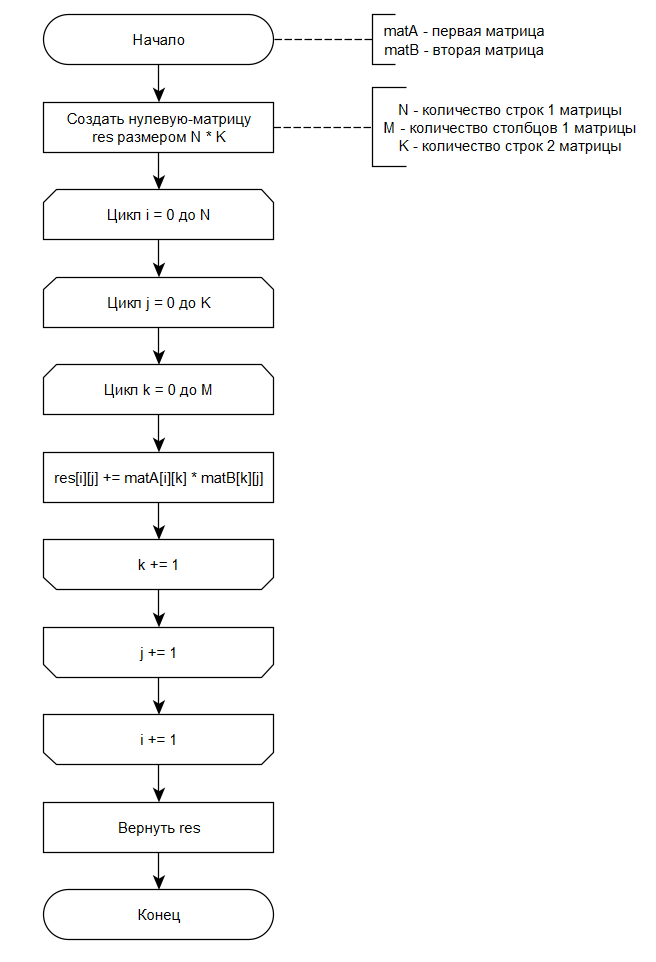
\includegraphics[scale=0.6]{tools/alg_1.png}
	\caption{Описание стандартного алгоритма умножения матриц}
	\label{fig:standard}
\end{figure}

\begin{figure}[h]
	\centering
	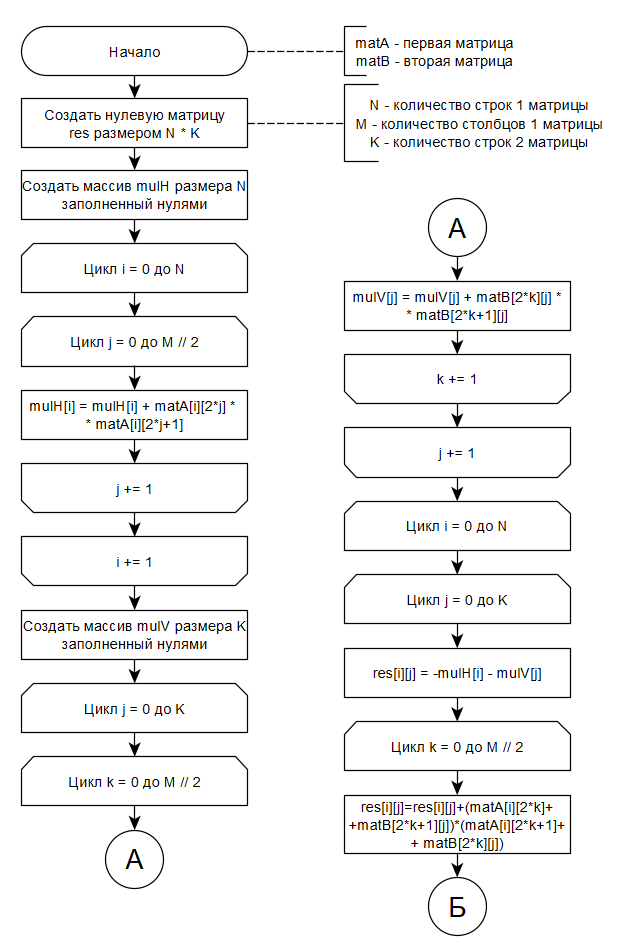
\includegraphics[scale=1]{tools/alg_2.png}
	\caption{Описание неоптимизированного алгоритма Винограда}
	\label{fig:vinograd_1}
\end{figure}

\begin{figure}[h]
	\centering
	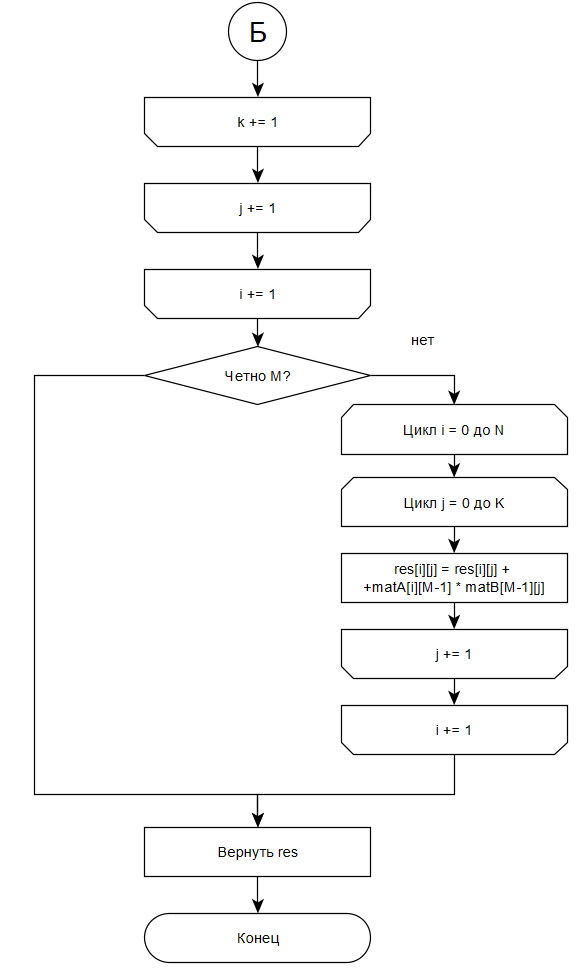
\includegraphics[scale=1]{tools/alg_2_1.png}
	\caption{Описание неоптимизированного алгоритма Винограда (продолжение)}
	\label{fig:vinograd_2}
\end{figure}

\begin{figure}[h]
	\centering
	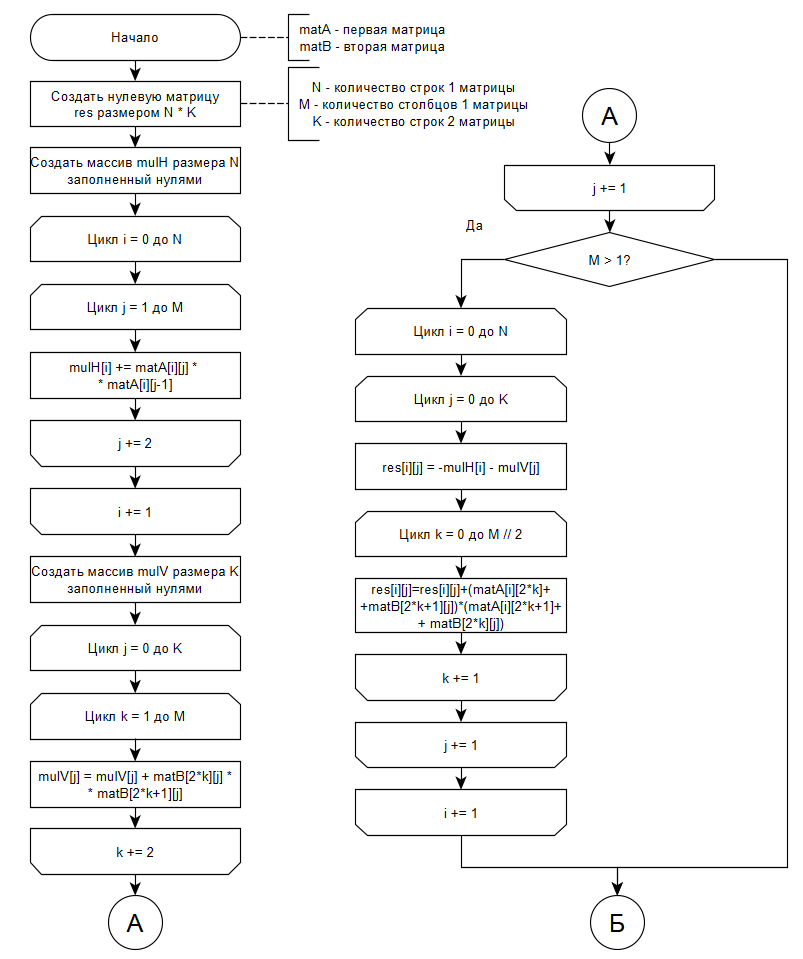
\includegraphics[scale=1]{tools/alg_3.png}
	\caption{Описание оптимизированного алгоритма Винограда}
	\label{fig:opt_vinograd_1}
\end{figure}

\begin{figure}[h]
	\centering
	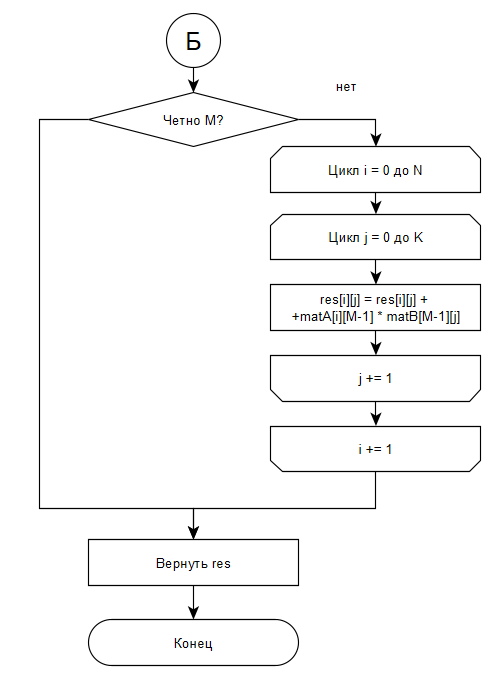
\includegraphics[scale=1]{tools/alg_3_1.png}
	\caption{Описание оптимизированного алгоритма Винограда (продолжение)}
	\label{fig:opt_vinograd_2}
\end{figure}

\clearpage\subsection{Модель вычислений}
Для вычисления трудоемкостей алгоритмов необходимо ввести модель вычислений:
\begin{enumerate}
	\item операции $+, -, [], ++, {-}-, ==, !=, <, >, <=, >=$ имеют трудоемкость 1;
	\item операции $*, /, \%, /=,  *=, \%=$ имеют трудоемкость 2;
	\item трудоемкость условного оператора \texttt{if <condition> then A else B} рассчитывается, как (\ref{eq:if});
	\begin{equation}
		\label{eq:if}
		f_{if} = f_{\text{condition}} +
		\begin{cases}
			f_A, & \text{если условие выполняется,}\\
			f_B, & \text{иначе.}
		\end{cases}
	\end{equation}
	\item трудоемкость цикла \texttt{for (init; condition; increment) \{ body \}} рассчитывается, как (\ref{eq:for})
	\begin{equation}
		\label{eq:for}
		f_{for} = f_{\text{init}} + f_{\text{condition}} + N\cdot(f_{\text{body}} + f_{\text{condition}} + f_{\text{increment}})
	\end{equation}
	где N -- количество итераций цикла;
	\item трудоемкость вызова функции равна 0.
\end{enumerate}

\clearpage\subsection{Вывод}
В этом разделе на основе теоретических аспектов были представлены описания стандартного алгоритма умножения матриц,
неоптимизированного алгоритма Винограда и оптимизированного алгоритма Винограда, который включает в себя следующие 
оптимизации:
\begin{enumerate}
	\item инкремент счётчика наиболее вложенного цикла на 2; 
	\item использование инкремента (+=); 
	\item вынос начальной итерации из каждого внешнего цикла.
\end{enumerate}
Так же была описана модель вычислений для дальнейшей оценки трудоемкости алгоритмов.


\clearpage\section{Технологическая часть}
В этом разделе обоснованы средства реализации, а так же представлены реализации алгоритмов, функциональные тесты
и оценки трудоемкостей алгоритмов.

\subsection{Средства реализации}
Для реализации алгоритмов в этой лабораторной работы был выбран язык $Python^{[2]}$, потому что в нем нет 
автоматического сборщика мусора. Время работы было замерено на микроконтроллерах $STM32^{[5]}$, с помощью функции
$ticks\_ms^{[1]}$ из библиотеки $time$ утилиты $MicroPython^{[3]}$. Запуск программы проводился утилитой $ampy^{[4]}$.

\subsection{Реализация алгоритмов}
В листингах \ref{lst:standard} - \ref{lst:opt_vinograd} представлены коды написанных алгоритмов.

\begin{lstlisting}[style=python, label=lst:standard,caption=Стандратный алгоритм умножения матриц]
def standard_mult(mat_a, mat_b):
    if len(mat_a) == 0 or len(mat_b) == 0:
        return []
    na = len(mat_a)
    ma = len(mat_a[0])
    nb = len(mat_b)
    mb = len(mat_b[0])
    if ma != nb:
        return []

    mat_c = [[0] * mb for i in range(na)]
    for i in range(na):
        for j in range(mb):
            for k in range(ma):
                mat_c[i][j] = mat_c[i][j] + mat_a[i][k] * mat_b[k][j]

    return mat_c
\end{lstlisting}

\clearpage\begin{lstlisting}[style=python, label=lst:vinograd,caption=Неоптимизированный алгоритм Винограда]
def vinograd_alg(mat_a, mat_b):
    if len(mat_a) == 0 or len(mat_b) == 0:
        return []
    na = len(mat_a)
    ma = len(mat_a[0])
    nb = len(mat_b)
    mb = len(mat_b[0])
    if ma != nb:
        return []

    mat_c = [[0] * mb for i in range(na)]

    mul_h = [0] * na
    for i in range(na):
        for j in range(ma // 2):
            mul_h[i] = mul_h[i] + mat_a[i][2 * j] * mat_a[i][2 * j + 1]

    mul_v = [0] * mb
    for j in range(mb):
        for k in range(nb // 2):
            mul_v[j] = mul_v[j] + mat_b[2 * k][j] * mat_b[2 * k + 1][j]

    for i in range(na):
        for j in range(mb):
            mat_c[i][j] = -mul_h[i] - mul_v[j]
            for k in range(ma // 2):
                mat_c[i][j] = mat_c[i][j] + (mat_a[i][2 * k] + mat_b[2 * k + 1][j]) * (mat_a[i][2 * k + 1] + mat_b[2 * k][j])

    if ma % 2 == 1:
        for i in range(na):
            for j in range(mb):
                mat_c[i][j] = mat_c[i][j] + mat_a[i][ma - 1] * mat_b[nb - 1][j]

    return mat_c
\end{lstlisting}

\clearpage\begin{lstlisting}[style=python, label=lst:opt_vinograd,caption=Оптимизированный алгоритм Винограда]
def optimized_vinograd_alg(mat_a, mat_b):
    if len(mat_a) == 0 or len(mat_b) == 0:
        return []
    na = len(mat_a)
    ma = len(mat_a[0])
    nb = len(mat_b)
    mb = len(mat_b[0])
    if ma != nb:
        return []

    mat_c = [[0] * mb for i in range(na)]

    mul_h = [0] * na
    for i in range(na):
        for j in range(1, ma, 2):
            mul_h[i] += mat_a[i][j] * mat_a[i][j - 1]

    mul_v = [0] * mb
    for j in range(mb):
        for k in range(1, nb, 2):
            mul_v[j] += mat_b[k][j] * mat_b[k - 1][j]

    if ma > 1:
        for i in range(na):
            for j in range(mb):
                mat_c[i][j] = (mat_a[i][0] + mat_b[1][j]) * (mat_a[i][1] + mat_b[0][j]) - mul_h[i] - mul_v[j]
                for k in range(2, ma - 1, 2):
                    mat_c[i][j] += (mat_a[i][k] + mat_b[k + 1][j]) * (mat_a[i][k + 1] + mat_b[k][j])

    if ma % 2 == 1:
        for i in range(na):
            for j in range(mb):
                mat_c[i][j] += mat_a[i][ma - 1] * mat_b[nb - 1][j]

    return mat_c
\end{lstlisting}

\clearpage\subsection{Функциональные тесты}
В таблице \ref{tbl:func_test} приведены функциональные тесты, на которых тестировалась программа.
\begin{table}[h]
	\begin{center}
	\caption{\label{tbl:func_test} Функциональные тесты, на которых были протестированы алгоритмы}
	\begin{tabular}{|c|c|c|}
		\hline
		Первая матрица  & Вторая матрица  & Результат
		\\ \hline
		Пустая матрица & Пустая матрица  & Сообщение об ошибке
		\\ \hline
		$\begin{pmatrix}
		1
		\end{pmatrix}$ &
		$\begin{pmatrix}
		2
		\end{pmatrix}$ &
		$\begin{pmatrix}
		2
		\end{pmatrix}$
		\\ \hline
		$\begin{pmatrix}
		1 & 2
		\end{pmatrix}$ &
		$\begin{pmatrix}
		2\\
		1
		\end{pmatrix}$ &
		$\begin{pmatrix}
		4
		\end{pmatrix}$
		\\ \hline
		$\begin{pmatrix}
		1 & 2
		\end{pmatrix}$ &
		$\begin{pmatrix}
		2
		\end{pmatrix}$ &
		Сообщение об ошибке
		\\ \hline
		$\begin{pmatrix}
		1\\
		2
		\end{pmatrix}$ &
		$\begin{pmatrix}
		2 & 1
		\end{pmatrix}$ &
		$\begin{pmatrix}
		2 & 1\\
		4 & 2
		\end{pmatrix}$
		\\ \hline
		$\begin{pmatrix}
		1 & 2 & 3\\
		3 & 2 & 1
		\end{pmatrix}$ &
		$\begin{pmatrix}
		2 & 1\\
		3 & 0\\
		4 & 2
		\end{pmatrix}$ &
		$\begin{pmatrix}
		20 & 7\\
		16 & 5
		\end{pmatrix}$
		\\ \hline
		$\begin{pmatrix}
		1 & 2 & 3\\
		4 & 5 & 6
		\end{pmatrix}$ &
		$\begin{pmatrix}
		1\\
		2\\
		3
		\end{pmatrix}$ &
		$\begin{pmatrix}
		14\\
		32
		\end{pmatrix}$
		\\ \hline
		$\begin{pmatrix}
		1 & 1\\
		1 & 1
		\end{pmatrix}$ &
		$\begin{pmatrix}
		1 & 1\\
		1 & 1
		\end{pmatrix}$ &
		$\begin{pmatrix}
		2 & 2\\
		2 & 2
		\end{pmatrix}$
		\\ \hline
		$\begin{pmatrix}
		1 & 0\\
		0 & 1
		\end{pmatrix}$ &
		$\begin{pmatrix}
		-1 & 0\\
		0 & -1
		\end{pmatrix}$ &
		$\begin{pmatrix}
		-1 & 0\\
		0 & -1
		\end{pmatrix}$
		\\ \hline
		$\begin{pmatrix}
		1 & 0\\
		0 & 1
		\end{pmatrix}$ &
		$\begin{pmatrix}
		0 & 0\\
		0 & 0
		\end{pmatrix}$ &
		$\begin{pmatrix}
		0 & 0\\
		0 & 0
		\end{pmatrix}$
		\\ \hline
	\end{tabular}
	\end{center}
\end{table}

\subsection{Оценка трудоемкости}
В этом разделе приведены оценки трудоемкостей алгоритмов согласно приведенным реализациям. При оценке алгоритма
в дальнейшем не будет учитываться проверка входных данных и инициализация результирующей матрицы, так как эти
действия являются общими во всех алгоритмах. Для рассчета трудоемкости примем $N = na, M = nb = ma, K = mb$.
\subsubsection{Стандартный алгоритм}
Трудоемкость стандартного алгоритма рассчитывается, как:
\begin{enumerate}
	\item цикла по i (12 строка), трудоемкость $f_{standard} = 2 + N \cdot (2 + f_{body_{i}})$;
	\item цикла по j (13 строка), трудоемкость $f_{body_{i}} = 2 + K \cdot (2 + f_{body_{j}})$;
	\item цикла по k (14 строка), трудоемкость $f_{body_{j}} = 2 + M \cdot (2 + f_{body_{k}}$;
	\item тело самого вложенного цикла (15 строка), трудоемкость $ f_{body_{k}} = 12$
\end{enumerate}
тогда $f_{standard} = 2 + N \cdot (4 + K \cdot (4 + 14M)) = 14MNK + 4NK + 4N + 2$

\begin{equation}
	\label{topic:standard}
	f_{standard} = 14MNK + 4NK + 4N + 2 \approx 10MNK
\end{equation}

\subsubsection{Неоптимизированный алгоритм Винограда}
Трудоемкость неоптимизированного алгоритма Винограда рассчитывается, как:
\begin{enumerate}
	\item инициализация нулями массивов mul\_h и mul\_v (13 и 18 строки), трудоемкость $f_{init} = N + K$;
	\item заполнение массива mul\_h (14-16 строки) $f_{inith} = 2 + N \cdot (2 + 4 + \frac{M}{2} \cdot (4 + 15) =
 \frac{19}{2}MN +6N + 2$;
	\item заполнение массива mul\_v (19-21 строки) $f_{initv} = 2 + K \cdot (2 + 4 + \frac{M}{2} \cdot (4 + 15) =
 \frac{19}{2}MK +6K + 2$;
	\item заполнение результирующей матрицы (23-27 строки) $f_{mult} = 2 + N \cdot (2 + 2 + K \cdot (2 + 7 + 4 + \frac{M}{2}
 \cdot (4 + 28) = 16MNK + 13NK +4N + 2$
 	\item проверка M на нечетность (29-32 строки) $f_{is} = \begin{cases} 3, & \text{четно,}\\
 													16NK + 4N + 5, & \text{иначе.}\end{cases}$
\end{enumerate}

\begin{equation}
	\label{topic:vinograd}
	f_{vinograd} = \begin{cases} 16MNK + 29NK + \frac{19}{2}MK + \frac{19}{2}MN + 15N + 7K + 11, & \text{х.с.,}\\
						16MNK + 13NK + \frac{19}{2}MK + \frac{19}{2}MN + 11N + 7K + 9, & \text{л.с.}
			    \end{cases}
\end{equation}

\subsubsection{Оптимизированный алгоритм Винограда}
Трудоемкость оптимизированного алгоритма Винограда рассчитывается, как:
\begin{enumerate}
	\item инициализация нулями массивов mul\_h и mul\_v (13 и 18 строки), трудоемкость $f_{init} = N + K$;
	\item заполнение массива mul\_h (14-16 строки) $f_{inith} = 2 + N \cdot (2 + 2 + \frac{M}{2} \cdot (2 + 9) =
 \frac{11}{2}MN +4N + 2$;
	\item заполнение массива mul\_v (19-21 строки) $f_{initv} = 2 + K \cdot (2 + 2 + \frac{M}{2} \cdot (2 + 9) =
 \frac{11}{2}MK +4K + 2$;
	\item заполнение результирующей матрицы (23-28 строки) $f_{mult} = 3 + N \cdot (2 + 2 + K \cdot (2 + 6 + 2 + \frac{M}{2}
 \cdot (2 + 17) = \frac{19}{2}MNK + 10NK +4N + 3$
 	\item проверка M на нечетность (30-33 строки) $f_{is} = \begin{cases} 3, & \text{четно,}\\
 													13NK + 4N + 5, & \text{иначе.}\end{cases}$
\end{enumerate}

\begin{equation}
	\label{topic:vinograd}
	f_{vinograd} = \begin{cases} \frac{19}{2}MNK + 23NK + \frac{11}{2}MK + \frac{11}{2}MN + 13N + 5K + 12, & \text{х.с.,}\\
					       \frac{19}{2}MNK + 10NK + \frac{11}{2}MK + \frac{11}{2}MN + 9N + 5K + 10, & \text{л.с.}
			    \end{cases}
\end{equation}

\subsection{Вывод}
В этом разделе на основе описаний алгоритмов были написаны и представлены коды алгоритмов. Помимо кодов
представлены функциональные тесты, на которых был протестирован каждый алгоритм. Так же приведена оценка
трудоемкости по модели вычислений, приведенной в предыдущей части. Согласно этой оценке наименьшая сложность
у оптимизированного алгоритма Винограда, затем у стандартного и только потом у неоптимизированного алгоритма
Винограда.


\clearpage\section{Исследовательская часть}
В этом разделе приведено сравнение по времени и по памяти написанных алгоритмов.

\subsection{Технические характеристики ЭВМ}
Все замеры проводились с помощью микроконтроллера STM32 на ЭВМ, характеристики которой приведены ниже:
\begin{itemize}
	\item Процессор -- 12th Gen Intel(R) Core(TM) i5-12450H   2.00 ГГц
	\item Оперативная память -- 16,0 ГБ
	\item Тип системы -- 64-разрядная операционная система, процессор x64
	\item Операционная система -- Windows 11
	\item Версия ОС -- 23H2
\end{itemize}

\subsection{Сравнение  по времени}
Время выполнения работы алгоритмов представлено в секундах. Проводилось 100 замеров.

\begin{table}[h]
	\begin{center}
	\caption{\label{tbl:all_time_cmp} Сравнение алгоритмов по времени выполнения}
	\begin{tabular}{|c|c|c|c|c|}
		\hline
		Размер квадратной матрицы & Стандартный & Виноград &  Оптимизированный
		\\ \hline
		20 & 0.0003 & 0.0001 & 0.0003
		\\ \hline
		40 & 0.002 & 0.002 & 0.002
		\\ \hline
		60 & 0.008 & 0.009 & 0.007
		\\ \hline
		80 & 0.019 & 0.019 & 0.014
		\\ \hline
		100 & 0.037 & 0.035 & 0.027
		\\ \hline
	\end{tabular}
	\end{center}
\end{table}

\begin{figure}[h]
	\centering
	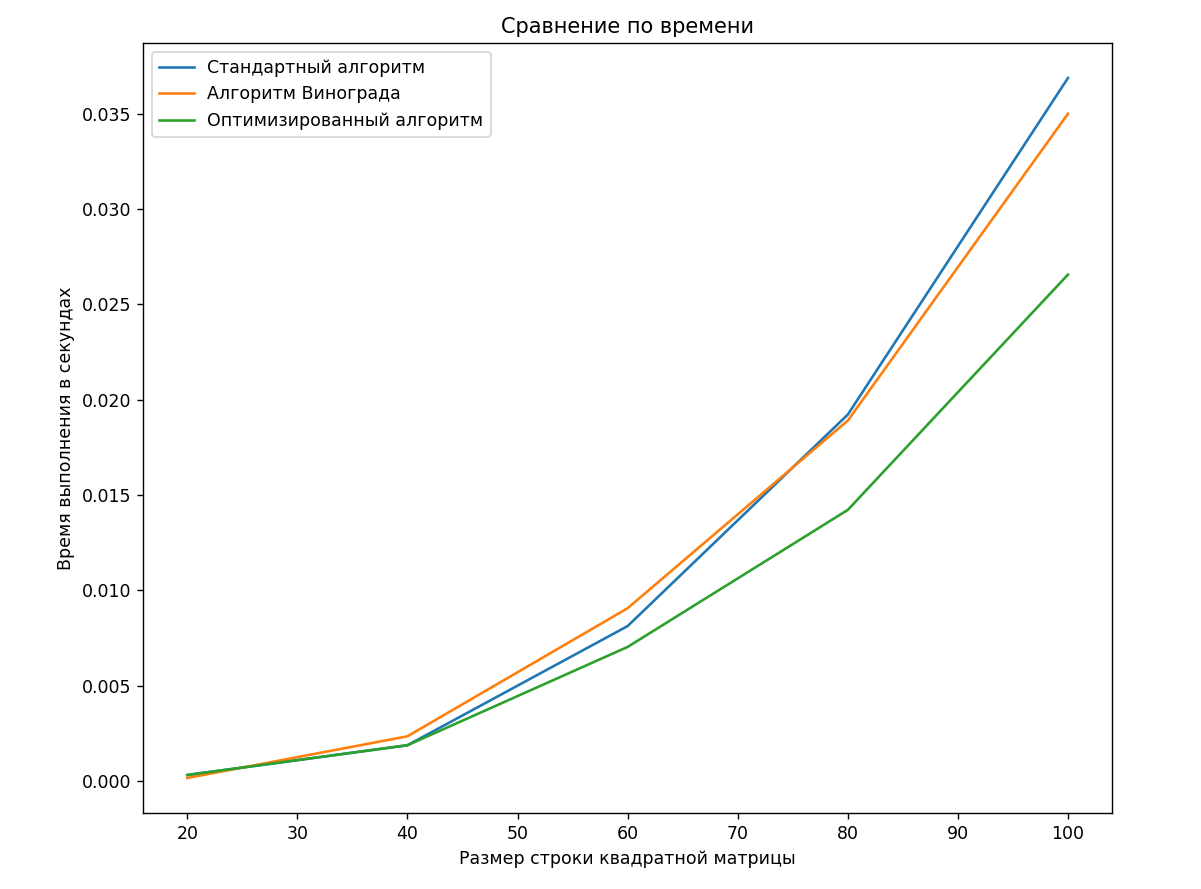
\includegraphics[scale=0.7]{tools/Screenshot_1.png}
	\caption{Сравнение алгоритмов по времени выполнения}
\end{figure}

\subsection{Вывод}
Неоптимизированный алгоритм Винограда, несмотря на большую теоретическую сложность, работает быстрее стандартного 
алгоритма. Алгоритм Винограда с оптимизацией работает быстрее всех алгоритмов примерно на 37\%.


\clearpage\section*{ЗАКЛЮЧЕНИЕ}
\addcontentsline{toc}{section}{ЗАКЛЮЧЕНИЕ}
В ходе выполнения лабораторной работы поставленная цель была достигнута, а также были решены следующие задачи:
\begin{itemize}
	\item описана математическая основа стандартного алгоритма умножения матриц и алгоритма Винограда;
	\item описана модель вычислений трудоемкости алгоритмов; 
	\item реализованы алгоритмы умножения матриц;
	\item выполнена оценка трудоемкости алгоритмов, согласно которой самый простой алгоритм -- оптимизированный
	алгоритм Винограда;
	\item проведено сравнение алгоритмов по времени:
	\begin{itemize}
		\item несмотря на свою большую сложность алгоритм Винограда работает быстрее стандартного алгоритма;
		\item самым быстрым оказался оптимизированный алгоритм Винограда;
	\end{itemize}
	\item описаны и обоснованы полученные результаты.
\end{itemize} 

\clearpage\section*{СПИСОК ИСПОЛЬЗОВАННЫХ ИСТОЧНИКОВ}
\addcontentsline{toc}{section}{СПИСОК ИСПОЛЬЗОВАННЫХ ИСТОЧНИКОВ}
\begin{enumerate}
	\item	Функция ticks\_ms -- https://docs.micropython.org/en/latest/library/time.html
	\item Welcome to Python -- https://www.python.org
	\item MicroPython --  https://docs.micropython.org
	\item Утилита ampy -- https://ampy.readthedocs.io/
	\item STM32 -- https://www.st.com/en/microcontrollers-microprocessors/\\
	stm32-32-bit-arm-cortex-mcus/documentation.html
\end{enumerate}

\end{document}